\documentclass{school-22.101-notes}
\date{December 13, 2011}

\begin{document}
\maketitle


\lecture{Final Review}

\topic{Introduction}
CGS unit: $\hbar c = 200 \fsp \MeV \cdot \fm$; the fine structure constant $\frac{e^2}{\hbar c} = \frac{1}{137}, m_n c^2 = 938.$
\begin{enumerate}
\item 
\eqn{ E_{\mathrm{ISW}} = \frac{Z_1 Z_2 e^2}{r^2} = \frac{Z_1 Z_2}{r^2} (\hbar c) \frac{e^2}{\hbar c} }
\item $mc^2$ for proton/neutron is about 940 MeV; electron is 0.5 MeV; reduced mass is $\frac{m_1 m_2}{m_1 + m_2}$. 
\eqn{ \frac{\hbar^2 \pi^2}{2 m L^2} = \frac{(\hbar c)^2 \pi^2}{2 (mc^2) L^2}   }
\item Alpha decay:
\eqn{ E_G = \left(\frac{2 \pi e^2 Z_{\alpha} Z_D}{\hbar c}\right)^2 \frac{\mu c^2}{2} = \left( \frac{2 \pi \cdot Z_{\alpha} Z_D}{137} \right)^2 \frac{m_{\alpha} m_D}{m_{\alpha} + m_D} \frac{938}{2} }
\end{enumerate}

%%%%%%%%%%%%%%%%%%%%%%%%% Topic 1 Quantum Mechanics %%%%%%%%%%%%%%%%%%%%%%%%%%%%
\topic{Schrodinger Equation}
\begin{enumerate}
\item Time-Independent Schrodinger Equation:
\begin{align}
\hat{H} \psi_n  &= E_n \psi_n  & 
- \frac{\hbar^2}{2m} \dpsidxn2 + V(x) \psi_n  &= E_n \psi_n \\
- \frac{\hbar^2}{2m} \dpsidxn2 + (V-E) \psi_n  &= 0  &
\dpsidxn2 + k^2 \psi_n  &=0, \fsp k = \sqrt{\frac{2 m (V-E)}{\hbar^2}}
\end{align}

\item Normalization:
\begin{align}
\int_{-\infty}^{\infty} |\psi(x)|^2 \dx &= 1 \\
\int_0^{\infty} 4 \pi r^2 \dr |\psi(r)|^2 &= 1 \\
\int_0^{2 \pi} \dpsi \int_0^{\pi} \sin \theta \dtheta |Y(\theta, \psi)|^2 &= 1 
\end{align}

\item Expectation: $ \expect{A} = \int_{-\infty}^{\infty} \psi^* A \psi \dx $.

\item Decompose wave function into bases: 
\begin{align}
\psi(x) &= \Sum_{n=1}^{\infty} C_n w_n (x) & \psi (x,t) &= \Sum_{n=1}^{\infty} C_n w_n(x) e^{ \frac{-iE_nt}{\hbar} } \\
P_n &= P(E_n) = |C_n|^2  & C_n &= \int \psi(x) w_n^* \dx
\end{align}

\item Ehrefest theory: $ \ddt \expect{A} = \frac{i}{\hbar} \expect{\left[ \Hhat, \Ahat \right] } + \overbrace{\expect{\ddt \Ahat}}^{\to 0} $. Application: $\ddt \expect{x} = \frac{1}{m} \expect{p}$. 

\item Position space: $\hat{p} = -i\hbar \ddx, \hat{H} = - \frac{\hbar^2}{2m} \nabla^2 + V(x) = \frac{\hat{p}^2}{2m} + V(x)$. 

\item Phase space: $\phat = \hbar k, \expect{E_n} = \frac{\hbar^2 k^2}{2m}$. Use Fourier transform to transfer $x$ space into $k$ space:
\eqn{ \phi(k) = \frac{1}{\sqrt{2\pi}} \int_{-\infty}^{\infty} e^{-ikx} \psi (x) \dx }

\item Common potentials: 

\begin{table}[h!]
    \centering
    \begin{tabular}{|p{1.4in}|c|c|c|} \hline
    Potential & Allowed energies & Wave forms & Wave bases\\ \hline
    ISW/Particle in a box & $E_n = \frac{n^2 \pi^2 \hbar^2}{2 m a^2} $ &  & $\psi_n (x) = \sqrt{\frac{2}{a}} \sin \left( \frac{n \pi x}{a} \right) $ \\ \hline
    \multirow{2}{*}{FSW} &  & $\psi(x) = A e^{ikx} + B e^{-ikx}, k = \frac{\sqrt{2m(E-V_1)}}{\hbar} $ & \\ 
     &  & $\psi(x) = C e^{\kappa x} + D e^{-\kappa x}, \kappa = \frac{\sqrt{2m(V_2 - E)}}{\hbar} $ & \\ \hline    
    Step Barrier, if $E>V$ & & $A e^{ik_1 x} + B e^{-ik_1 x}, Ce^{ik_2x} $   & \\ \hline
    Step Barrier, if $E<V$ & & $A e^{ik_1 x} + Be^{-ik_1 x}, C e^{-\kappa x}$ & \\ \hline
    Rectanger Step Barrier & & $A e^{i k_1 x} + B e^{-ik_1 x}, Ce^{\kappa x} + D e^{-\kappa x}, E e^{ik_1 x}$ & \\ \hline
    \end{tabular}
    \caption{Common Potentials}
\end{table}

Notice, $e^{ikx}$ means traveling to the right, $e^{-ikx}$ means traveling to the left. For calculating $T, R$, we do the ratio of flux, which is defined as: $\Gamma = |\psi|^2 \frac{\hbar k}{m}$. 

\end{enumerate}

\topic{Angular Momentum} 
\begin{align}
L^2 &= L_x^2 + l_y^2 + L_z^2 & [ \hat{L}_x, \hat{L}_y ] &= i \hbar \hat{L}_z \\
L^2 \psi &= \hbar^2 l (l+1) \psi & L_z \psi &= \hbar m \psi \\
[\hat{x}, \hat{p} ] &= i \hbar & [\hat{L}^2, \hat{H} ] &= 0 \\
[ \hat{x}, \hat{p}^2] &= [\hat{x}, \hat{p} ] \hat{p} + \hat{p} [\hat{x}, \hat{p} ]  = 2 i \hbar \hat{p} & [\hat{x}^2, \hat{p} ] &= \hat{x} [\hat{x}, \hat{p} ] + [\hat{x}, \hat{p} ] \hat{x} = 2 i \hbar \hat{x} \\
\ddt \expect{\hat{x}} &= \frac{\expect{\hat{p}}}{m} & \ddt \expect{\hat{p}} &= - \expect{ \dVdx }
\end{align}

\uline{Radial Schroedinger Equation:} 
\begin{align}
\mathrm{Define} \fsp \fsp u_{nl} (r) &= r \psi_{nl} (r) \\ 
\left[ - \frac{\hbar^2}{2m} \ddrn2 + \overbrace{\frac{\hbar^2 l (l+1)}{2 \mu r^2} + V_{\mathrm{nuc}} (r) }^{V_{\mathrm{eff}} (r)} - E \right] u_{nl} (r) &= 0 
\end{align}
Eigenstate for $\hat{L}^2, \hat{L}_z, \hat{H}$ is the spherical harmonics $Y_l^m (\theta, \phi)$. 

The $\frac{\hbar^2 l(l+1)}{2 \mu r^2}$ term weaken the well. For n-p scattering, $V_{\mathrm{nuc}} (r) = V_0 (r) + V_1 (r) \frac{\shat_p \cdot \shat_n}{\hbar^2}$. 
To find $\expect{\lhat \cdot \shat}$: 
\begin{align}
\jhat^2 &= (\lhat + \shat)(\lhat + \shat) = \lhat^2 + \shat^2 + 2 \lhat \cdot \shat \\ 
\lhat \cdot \shat &= \frac{1}{2} (\jhat^2 - \lhat^2 - \shat^2 ) \\
\expect{ \lhat \cdot \shat} &= \frac{\hbar^2}{2} \left[ j(j+1) - l(l+1) - s(s+1) \right] \\
\expect{ \shat_p \cdot \shat_n} &= \frac{\hbar^2}{2} \left[ s(s+1) - s_p(s_p+1) - s_n(s_n+1) \right] 
\end{align}
\uline{Singlet vs. Triplet} 
Following the expressions in Radial Schroedinger Equation section, we can write: 
\begin{align}
\begin{dcases*}
V_{\mathrm{nuc,T}} = V_0 + \frac{1}{4} V_1 & Triplet, bounded (well deeper) \\
V_{\mathrm{nuc,S}} = V_0 - \frac{3}{4} V_1 & Singlet, unbound (well weaker)
\end{dcases*}
\end{align}
Using notation for $\ket{s m}$ \footnote{Griffiths p185}: 
\begin{align}
\left\{ \begin{array}{l} 
\ket{1 1} = \up \up \\
\ket{1 0} = \frac{1}{\sqrt{2}} (\up \down + \down \up ) \\
\ket{1 -1} = \down \down
\end{array} \right\}
S = 1 (\mathrm{triplet, parallel, bounded}). \\
\left\{ \ket{0 0} = \frac{1}{\sqrt{2}} (\up \down - \down \up ) \right\} 
S = 0 (\mathrm{singlet, anti-parallel, unbounded}).
\end{align}
Beyond this, we need the Clebsch-Gordan coefficients table to find the coefficients in 
\eqn{\ket{s m} = \Sum_{m_1 + m_2 = m} C_{m_1 m_2 m}^{s_1 s_2 s} \ket{s_1 m_1} \ket{s_2 m_2} }
\uline{Deuteron Example:} 
    \begin{enumerate}
    \item $l=0$ is the only bound state because: $V_{\mathrm{eff}} = V + \frac{\hbar^2 l(l+1)}{2 \mu r_0^2}$. 
    \eqn{ \Delta V = \frac{\hbar^2 l(l+1)}{2 \mu r_0^2} = \frac{(\hbar c)^2 l(l+1)}{2 (\mu c^2) r^2} = \frac{(200)^2 l(l+1)}{2 (500)(2.1)^2} = 10 l(l+1) \fsp \MeV   }
    For $l=1, \Delta V = 20 \fsp \MeV > E_B = 2.2 \fsp \MeV$.
    \item Spin-spin coupling is necessary, because 
    \eqn{ V_{\mathrm{eff}} = V_0 + V_1 \frac{\expect{\hat{s}_p \cdot \hat{s}_n}}{\hbar^2} = V_0 + \frac{V_1}{2} \left[ s(s+1) - \frac{3}{2} \right] = \left\{ \begin{array}{cc} V_0 - \frac{3}{4} V_1 & S=0 \mbox{ Singlet} \\ V_0 + \frac{1}{4} V_1 & S = 1 \mbox{ Triplet}  \end{array} \right.   }
    We are given $V_T = 35$ MeV, use the `barely bound state' to find $V_S$: 
    \eqn{ \frac{\lambda}{4} = r_0 \Rightarrow k = \frac{2\pi}{\lambda} = \frac{\pi}{2 r_0}, V_S \sim E+ V_S = \frac{\hbar^2 k^2}{2m} = \frac{\hbar^2}{2m} k^2 = \frac{\hbar^2}{2m} \frac{\pi^2}{4 r_0^2} \sim 22 \fsp \MeV.}
    We plug in $V_T = 35 \fsp \MeV, V_S = 22 \fsp \MeV$ to find that $V_0 = 32 \fsp \MeV, V_1 = 13 \fsp \MeV$. 
    \item $l>0$ can only exist for $s=1$, singlet well is less deep than triplet.     
    \end{enumerate}
\clearpage
%%%%%%%%%%%%%%%%%%%%%%%%% Topic 2 Nuclear Structure %%%%%%%%%%%%%%%%%%%%%%%%%%%%
\topic{Nuclear Structure}

\uline{Scattering}
\begin{enumerate}
\item 
    \begin{align}
        \psi (r) &= \overbrace{e^{i  (k z - wt)}}^{\mathrm{incoming}} + \overbrace{ f(\theta) \frac{e^{i (k r - wt)}}{r} }^{\mathrm{outgoing}} 
        &  \dsigmadOmega &= |f(\theta)|^2 = (\mathrm{scattering \fsp amplitude})^2 \\
        \psi(r,\theta) &= \Sum_{l=0}^{\infty} R_l (r) P_l (\cos \theta) 
        &  u_l (r) &= \frac{a_l}{k} \sin \left( kr - \frac{l \pi}{2} + \delta_l \right) 
    \end{align}
%    
\item We plug $u_l(r)$ back into partial wave $\psi(r,\theta)$, in which Legende Polynomial $P_0 = 1, P_1 = \cos \theta$:
\eqn{ \psi(r,\theta) = \Sum_{l=0}^{\infty} \frac{a_l}{kr} \sin \left( kr - \frac{l \pi}{2} + \delta_l \right) P_l (\cos \theta)  }
%
\item We equate the coefficients of the same term: 
\begin{align}
f(\theta) &= \frac{1}{k} \Sum_{l=0}^{\infty} (2l+1) e^{i \delta_l} \sin \delta_l P_l (\cos \theta) \\
\sigma (\theta) &= |f(\theta)|^2 =  \frac{1}{k^2} \Sum_{l=0}^{\infty} (2l+1) e^{i \delta_l} \sin^2 \delta_l 
\end{align}
%
\item Low Energy Scattering (S-Wave Approximation): assume $E$ is small, then $k,r$ is small; we can derive $l < kr_0 \ll 1$, hence $l=0$ for low energy S-wave approximation
\eqn{ \boxed{ u_0 (r) = \frac{a_0}{k} \sin (kr + \delta_0), \fsp \sigma(\theta) = \frac{1}{k^2} \sin^2 \delta_0, \fsp \sigma = 4 \pi \sigma(\theta) } }
Notice $f(\theta), \sigma (\theta), \theta$ do not depend on $\theta$. Keep in mind that $\psi = \frac{u}{r}$, hence for S-wave, $\psi \sim \frac{\sin (kr + \delta)}{kr}$.
%
\item To use S-wave approximation, given a potential well of $-V_0$, inside of the well assume $u(r) = B \sin (kr)$, outside assume $u(r) = A \sin(kr + \delta_0)$. Then solve for $\delta_0$.
%
\item Scattering length $a$: it behaves like an intercept. Bound state $a>0$, unbound state $a<0$.  
\begin{align}
- \lim_{k \to 0} f(\theta) &= a & \delta_0 &= -ak \\
\sigma (\theta) &= \frac{\sin^2 (\delta_0)}{k^2} \approx \frac{\delta_0^2}{k^2} =  a^2 & u(r) &= \frac{a_0}{k} (k (r-a)) 
\end{align} 
\begin{figure}[ht]
    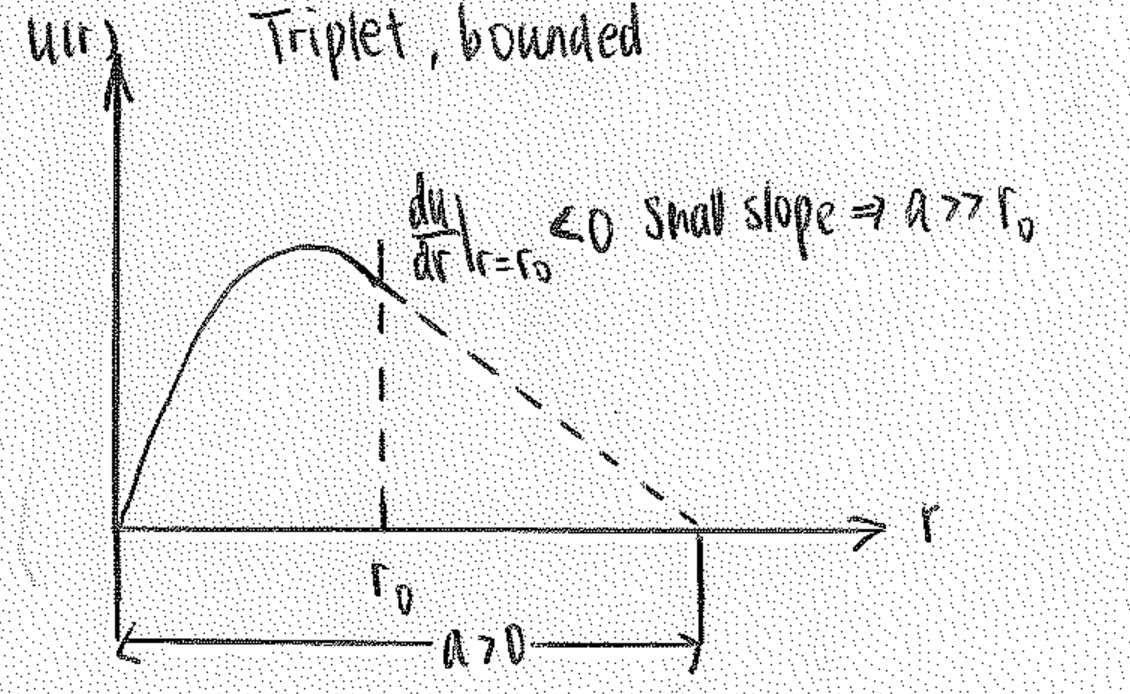
\includegraphics[width=3in]{images/scattering/s-wave-triplet.png}
    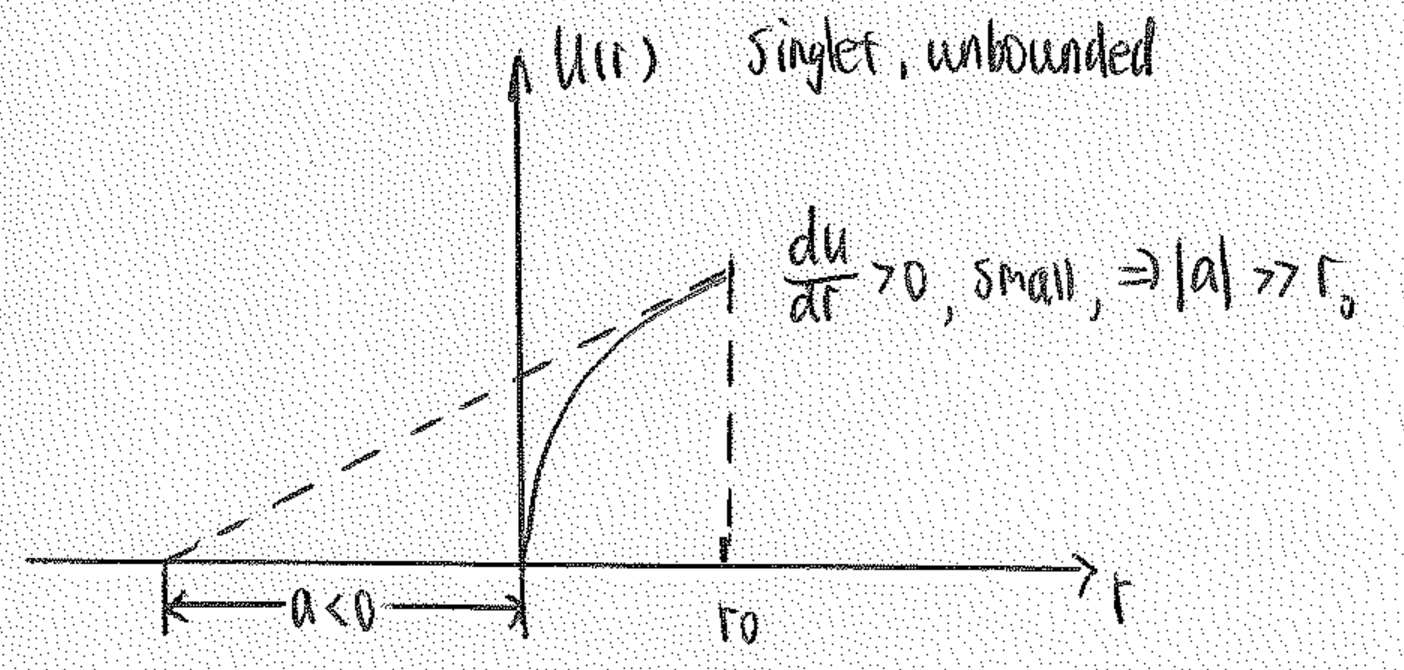
\includegraphics[width=3in]{images/scattering/s-wave-singlet.png}    
\end{figure}
%
\item Know that negative potential is attractive, pulling the wave function in, $\delta_0 >0$, vise versa (recall the graph). 
%
\item Applying S-wave to n-p scattering
\begin{align}
\sin^2 (\delta_0) &= \frac{1}{1 + \left( \frac{k_2^B}{k_2} \right)^2 } \\
\sigma &= \frac{4\pi}{k^2} \sin^2 (\delta_0) = \frac{4\pi}{k_2^2 + \left(k_2^B \right)^2 } = \frac{4\pi \hbar^2}{2 \mu (E + E_B) } \xrightarrow{E \ll E_B} \frac{4 \pi \hbar^2}{2 \mu} \frac{1}{E_B} 
\end{align}
Plug in $E_B = 2.22$ MeV, we get $\sigma = 2.3$ b, which is significantly smaller than the 20 b measured. The missing piece is the spin-spin coupling:
\begin{align}
\sigma( \theta) &= \frac{3}{4} \sigma_T (\theta) + \frac{1}{4} \sigma_S (\theta) = \frac{3}{4} \frac{1}{k_2^2} \sin^2 (\theta_{ot} ) + \frac{1}{4} \frac{1}{k_2^2} \sin^2 (\theta_{os} ) \\
\sigma &= 4 \pi \sigma (\theta) = \frac{4 \pi \hbar^2}{2 \mu} \left[ \frac{3}{4} \frac{1}{E_B} + \frac{1}{4} \frac{1}{E^*} \right] 
\end{align}
Plug in $E_B = 2.22 \fsp \MeV, E^* = 0.077 \fsp \MeV$, $\sigma = 19$ b, which is a good approximation for 20b.
%
%
\item In nuclear interaction section, we talked about:
    \begin{align}
    \cos \theta &= \frac{1+ A \cos \theta_C}{\sqrt{A^2 + 1 + 2A \cos \theta_C} } \\
    \frac{E^{\prime}}{E} &= \frac{A^2 + 2A \cos \theta_C + 1}{(A+1)^2} \\
    \expect{ \frac{E^{\prime}}{E} } &= \frac{(A-1)^2}{(A+1)^2} = \alpha 
    \end{align}
    know $P(\mu)$ graph, know $P(E \to E^{\prime})$ graph.
\end{enumerate}


\clearpage
\uline{Shell Model}
\begin{enumerate}
\item Nuclear Magic Number(Z or N): 2 (He), 8 (Oxygen), 20, 28, 50 (Zr), 82, 126. 
\item Evidence of nuclear magic number and shell model:
\begin{enumerate}
\item Abundance of stable isotones (Isotones: same neutron number N, but different proton number Z; Isotopes: same proton number Z, but different neutron number N) is large (by 5 to 7 times) for nuclei with magic number of neutrons.
\begin{figure}[ht]
  \centering
  \subfloat[Evidence 1]{\label{fig:111}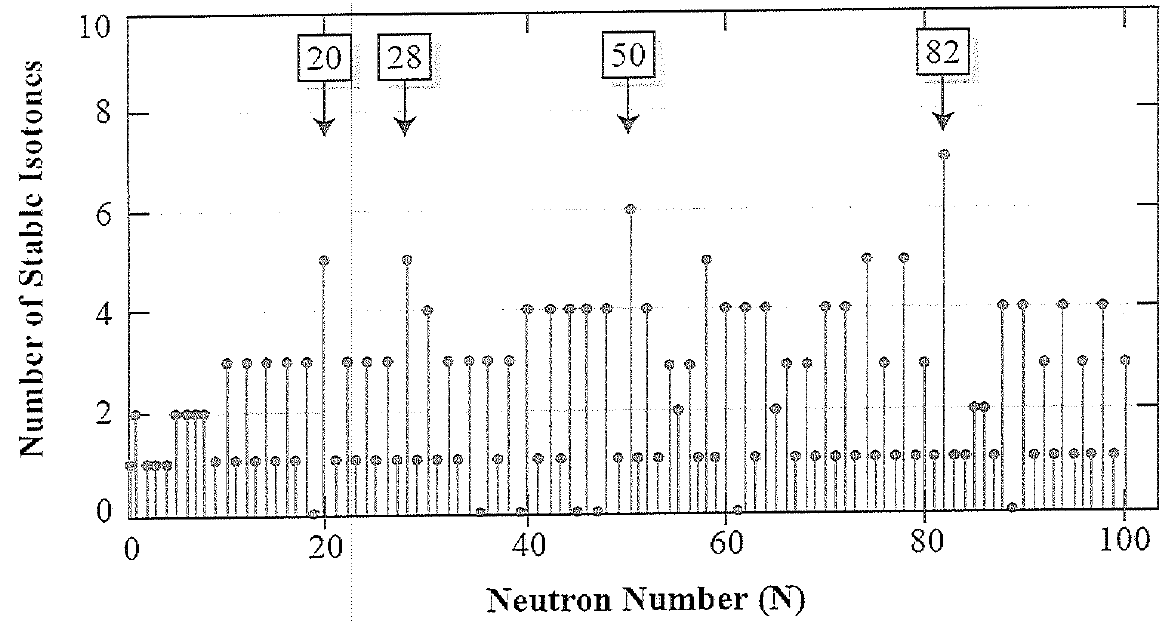
\includegraphics[width=0.5\textwidth]{images/shell/shell-evidence-1.png}}    
  \subfloat[Evidence 2]{\label{fig:112}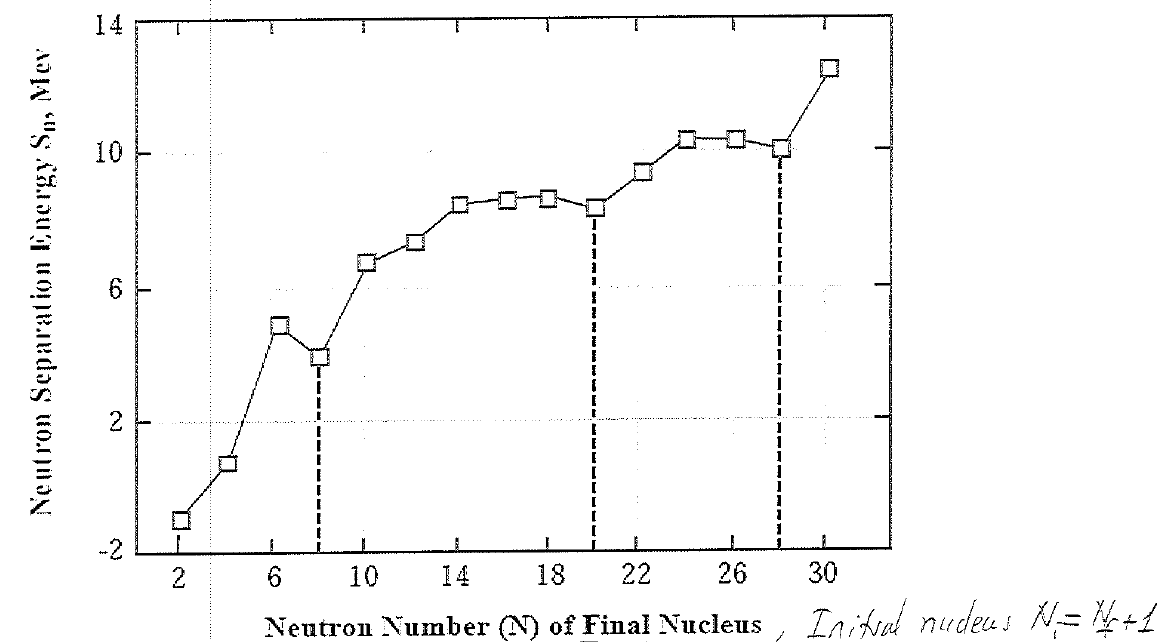
\includegraphics[width=0.5\textwidth]{images/shell/shell-evidence-2.png}}                              
\end{figure}
\item Neutron separation energy $S_n$ is low for nuclei with one more neutron than a magic number. Reason: it is easier to separate one neutron when number of neutrons is magic plus 1; that is, magic neutron numbers are more tightly bound \footnote{Also see Krane Figure 5.2}. 
\item The first excited states of even-even nuclei have higher than usual energies at magic numbers because, again, these nuclei are tightly bound. If tightly bound, then excite energy increases. 
\begin{figure}[ht]
  \centering
  \subfloat[Evidence 3]{\label{fig:113}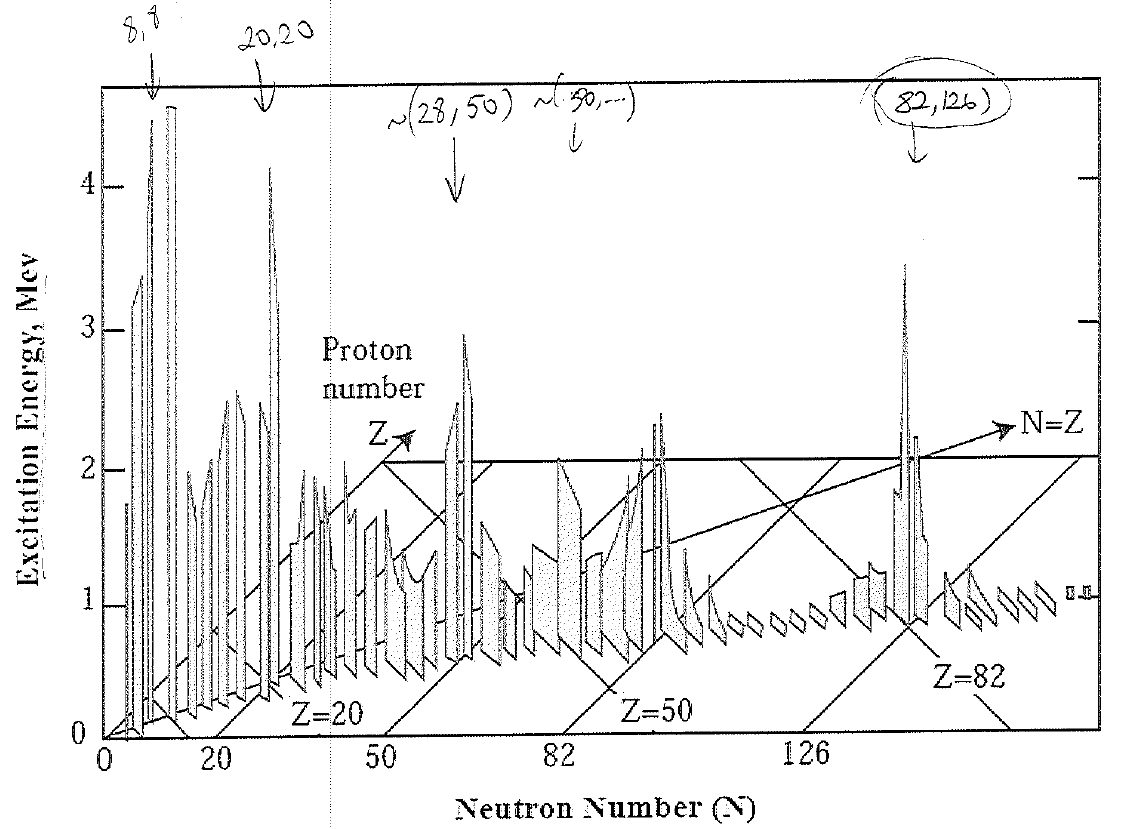
\includegraphics[width=0.5\textwidth]{images/shell/shell-evidence-3.png}}    
  \subfloat[Evidence 4]{\label{fig:114}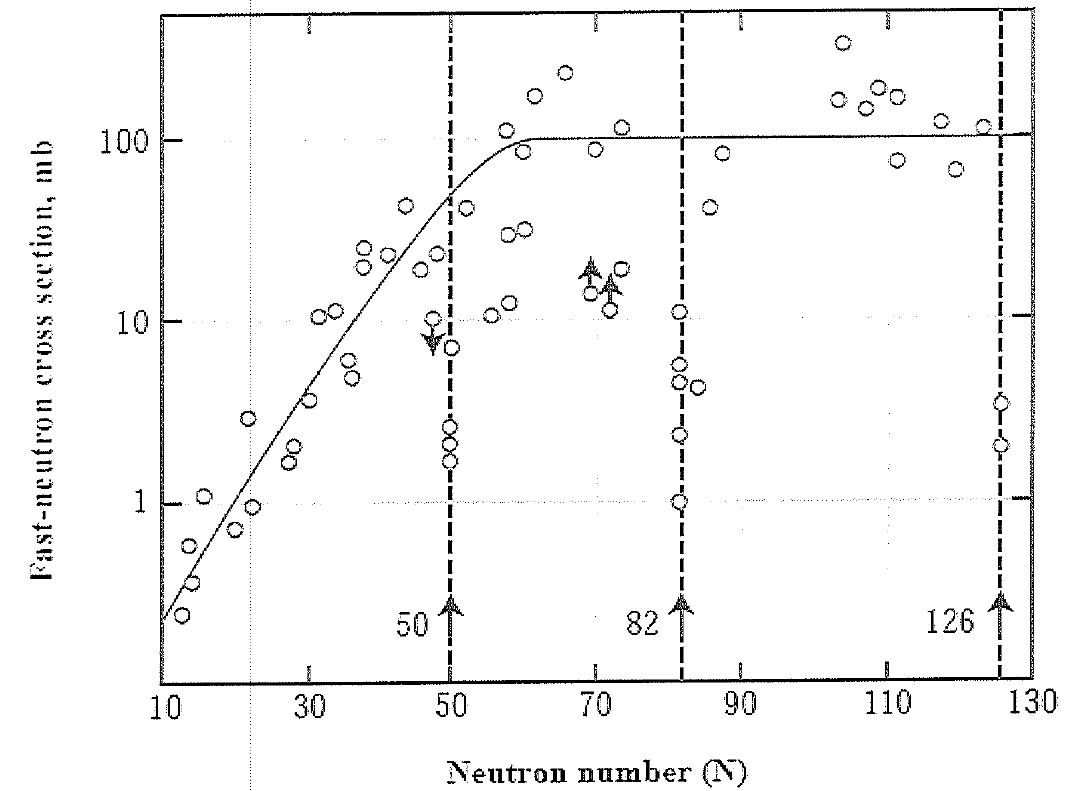
\includegraphics[width=0.5\textwidth]{images/shell/shell-evidence-4.png}}                              
\end{figure}
\item Neutron capture cross sections are low for these numbers: they are stable already, do not want to absorb neutron. Zr has Z=40 and has about 50,51,52 neutrons, hence it is `neutron transparent.'
\item Nuclear charge radius decreases and then suddenly jumps at magic numbers. 
\begin{figure}[ht]
    \centering
    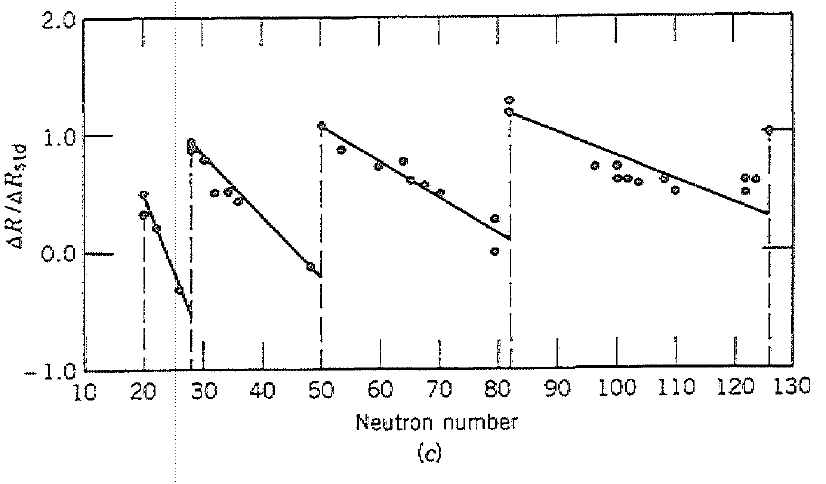
\includegraphics[width=3in]{images/shell/shell-evidence-5.png}
\end{figure}
\end{enumerate}

\item Potential Model 1: Infinite Wall. It does not work because it requires infinite amount of energy to separate a neutron or a proton; model has sharp edge, whereas nuclear charge and matter distribution fall smoothly to zero beyond the mean radius. 

\item Potential Model 2: Harmonic Oscillator: It does not work because the energy goes to infinity, and the potential inside of the well is not sharp enough (compare with experimental results);
    \begin{enumerate}
    \item Unmodified Harmonic Oscillator: $V_{\mathrm{eff}}$ takes the general form of $V_{\mathrm{eff}} = \frac{1}{2} m \omega^2 r^2 - V_0^{\prime},$ 
        \begin{align}
        \omega^2 =
        \begin{dcases*}
        \frac{2}{m} \frac{V_0}{R_0^2}  & neutrons \\
        \frac{2}{m} \left[ \frac{V_0}{R_0^2} - \frac{(Z-1) e^2}{2 R_0^3} \right] & protons \\
        \end{dcases*}
        \fsp \fsp \fsp \fsp \fsp
        V_0^{\prime} = 
        \begin{dcases*}
        V_0 & neutrons \\
        V_0 - \frac{3}{2} \frac{(Z-1) e^2}{R_0} & protons \\
        \end{dcases*}
        \end{align}
    Harmonic Oscillator Energy Eigenvalues are:
        \eqn{ E_n = \hbar \omega \left( n + \frac{3}{2} \right) - V_0^{\prime} }
    The allowed quantum numbers are:    
        \begin{enumerate}
            \item Given the Oscillator Level $n$, $l$ has to satisfy: $ l \le n, \mbox{l has same even-odd-ness as n.}$
            \item Knowing $l$, $-l \le m_l \le l$, hence $2l+1$ degeneracy, also take into account $m_s = \pm \frac{1}{2}$, then the total degeneracy is $ D_l (l) = 2l+1, \fsp D_{l,s} (l) = 2(2l+1) = 4l+2$.
            \item Written $D_{l,s}$ as a function of $n$, the total number of degeneracy is: 
            $ D_l (n) = \frac{1}{2} (n+1)(n+2), \fsp D_{l,s} (n) = (n+1)(n+2).$
        \end{enumerate}
    Two problems with this model: total \# of allowed energies are correct for $n=0,1,2$ but off for the rest; Separation energy $\Delta E$ predicted is larger than reality.        
        
    \item Modified Harmonic Oscillator: know the degeneracy graph and find $\Delta E$. 
        \eqn{ V_{\mathrm{nuc}} = V_0 + V_{\mathrm{so}} \frac{\hat{l} \cdot \hat{s} }{\hbar^2} }  
    \begin{align}
        \expect{\lhat \cdot \shat} &= \frac{\hbar^2}{2} \left[ j(j+1) - l(l+1) - \frac{3}{4} \right] 
        =
        \begin{dcases*}
        - \frac{\hbar^2}{2} (l+1) & for $j = l-\frac{1}{2}$. \\ 
        \frac{\hbar^2}{2} l & for $j = l + \frac{1}{2}$. \\
        \end{dcases*} 
        \\
        V_{\mathrm{nuc}} (r) &= 
        \begin{dcases*}
        V_0 - \frac{l+1}{2} V_{\mathrm{so}} & for $j = l-\frac{1}{2}$. \\ 
        V_0 + \frac{l}{2} V_{\mathrm{so}} & for $j = l + \frac{1}{2}$. \\
        \end{dcases*}
    \end{align}
    Keep in mind that $V_0 < 0, V_{\mathrm{so}} < 0$, so 
    \begin{itemize}
        \item $j = l+\frac{1}{2}$: pushes the well and the energy levels down (lower), more tightly bound; the attractive well is more attractive; 
        \item $j = l - \frac{1}{2}$: pushes the well and the energy levels higher (up), more weakly bound.  
    \end{itemize}    
     For a pair of states with $l>0$, the energy splitting difference increases with increasing $l$:
\eqn{ \Delta E = \expect{ \lhat \cdot \shat }_{j = l+\frac{1}{2} } - \expect{ \lhat \cdot \shat }_{j = l-\frac{1}{2} } = \frac{\hbar^2}{2} (2l+1) }
The physical interpretation of the this is that states with larger $l$ values split more; for instance, $1f$ state split more than than $2p$. In the deuteron example, $l=0$, hence we do not consider spin-orbit coupling.               
    \end{enumerate}
\end{enumerate}


\uline{Spin-Parity Assignment}
\begin{enumerate}
\item odd p, even n: $I^{\pi}$ of unpaired p;
\item odd n, even p: $I^{\pi}$ of unpaired n;
\item even-even: $I^{\pi} = 0^+$;
\item odd-odd: 
    \begin{enumerate}
    \item parity opposite: $I = |I_p - I_n|$;
    \item parity same: $I = I_p + I_n$;
    \item $\pi = (-1)^{L_p} (-1)^{L_n}$. 
    \end{enumerate}
\end{enumerate}



\clearpage
%%%%%%%%%%%%%%%%%%%%%%%%% Topic 3 Radioactive Decay %%%%%%%%%%%%%%%%%%%%%%%%%%%%
\topic{Radioactive Decay}

\uline{Binding energy, stability, mass parabola.}
\begin{enumerate}
\item Stability's governing factor: nuclear mass. Typically, a higher B/A means more stable.
\item Binding energy of a nucleus with A,Z:
\begin{align} 
B(A,Z) &= \left[ Z m_p + N m_n - (m(A,Z) - Z m_e) \right] c^2 \\
&= \left[ Z m_{\ce{^1 H}} + N m_n - m(A,Z) \right] c^2
\end{align}
\item Binding energy for the outmost neutron (`valence' nucleon) $=$ neutron separation energy $=$ the energy required to separate one neutron from a nucleus; similarly for proton separation energy: 
\begin{align}
S_n &= B(\ce{^A_Z X_N}) -B(\ce{^{A-1}_Z X_{N-1}}) = \left[ m(A-1, Z) - m(A,Z) + m_n \right] c^2 \\
S_p &= B(\ce{^A_Z X_N}) -B(\ce{^{A-1}_{Z-1} X_{N}}) = \left[ m(A-1, Z-1) - m(A,Z) + m_{H} \right] c^2
\end{align}
\item Semi-empirical binding energy formula:
    \eqn{B = \underbrace{15.5 A - 16.8 A^{2/3} - 0.72 \frac{Z(Z-1)}{A^{1/3}}}_{\mbox{`liquid-drop model,' collective behavior.}} \underbrace{- 23 \frac{(A-2Z)^2}{A} \pm 34 A^{-3/4}}_{\mbox{`shell model,' individual nucleon behavior.}}   }
    Parity Contribution: this term arises from the tendency of the like nucleons (neutron \& neutrons, protons \& protons) to couple pairwise to more stable configurations.
    \begin{enumerate}
    \item Odd N, odd Z: weakly bound, lose binding energy, $\sim -a_p A^{-3/4}$;
    \item Odd A: no effect;
    \item Even N, even Z: tightly bound, gain binding energy, $\sim a_p A^{-3/4}$.
    \end{enumerate}
\item Binding energy per nucleon graph: initial rise in B/A is due to decreasing importance of the surface term as A increases. The peak at A=60 is due to Coulomb repulsion increases as A increases.     
\item SEMF: combine the two formulas we have about binding energy. 
\begin{align}
B(A,Z) &= \left[ Z m_H + N m_n - m(A,Z) \right] c^2  \label{BAZ}\\
m(A,Z) c^2 &= \left[ Z m_H + N m_n \right] c^2 - B(A,Z) = Z^2 (\cdots) + Z(\cdots) + C \label{SEMF-m}
\end{align}
\item Mass parabola is derived from Eq.~\ref{SEMF-m}. $\frac{\dM}{\dZ} = 0$ to find $Z_{\mathrm{min}}$. At small A, $Z_{\mathrm{min}} \sim \frac{A}{2}$. At large A, $Z_{\mathrm{min}} < \frac{A}{2} \sim 0.41 A$. 
\eqn{ Z_{\mathrm{min}} \approx \frac{A/2}{1 + \frac{1}{4} \frac{a_c}{a_{\mathrm{sym}}} A^{3/4}} }
\item Mass parabola is used for: 
    \begin{enumerate}
    \item To determine whether a decay process will happen or not, it has to be \textcolor{blue}{energetically allowed, $M_{\mathrm{final}} < M_{\mathrm{initial}}$, that is, goes down on the M vs. Z curve.}
    \item Remember for odd A there is only 1 parabola; for even A there are two (o-o is above e-e)
    \end{enumerate}
\end{enumerate}

\clearpage
\uline{Decays}

\begin{enumerate}
\item Common decay types:
    \begin{figure}[h!]
        \centering
        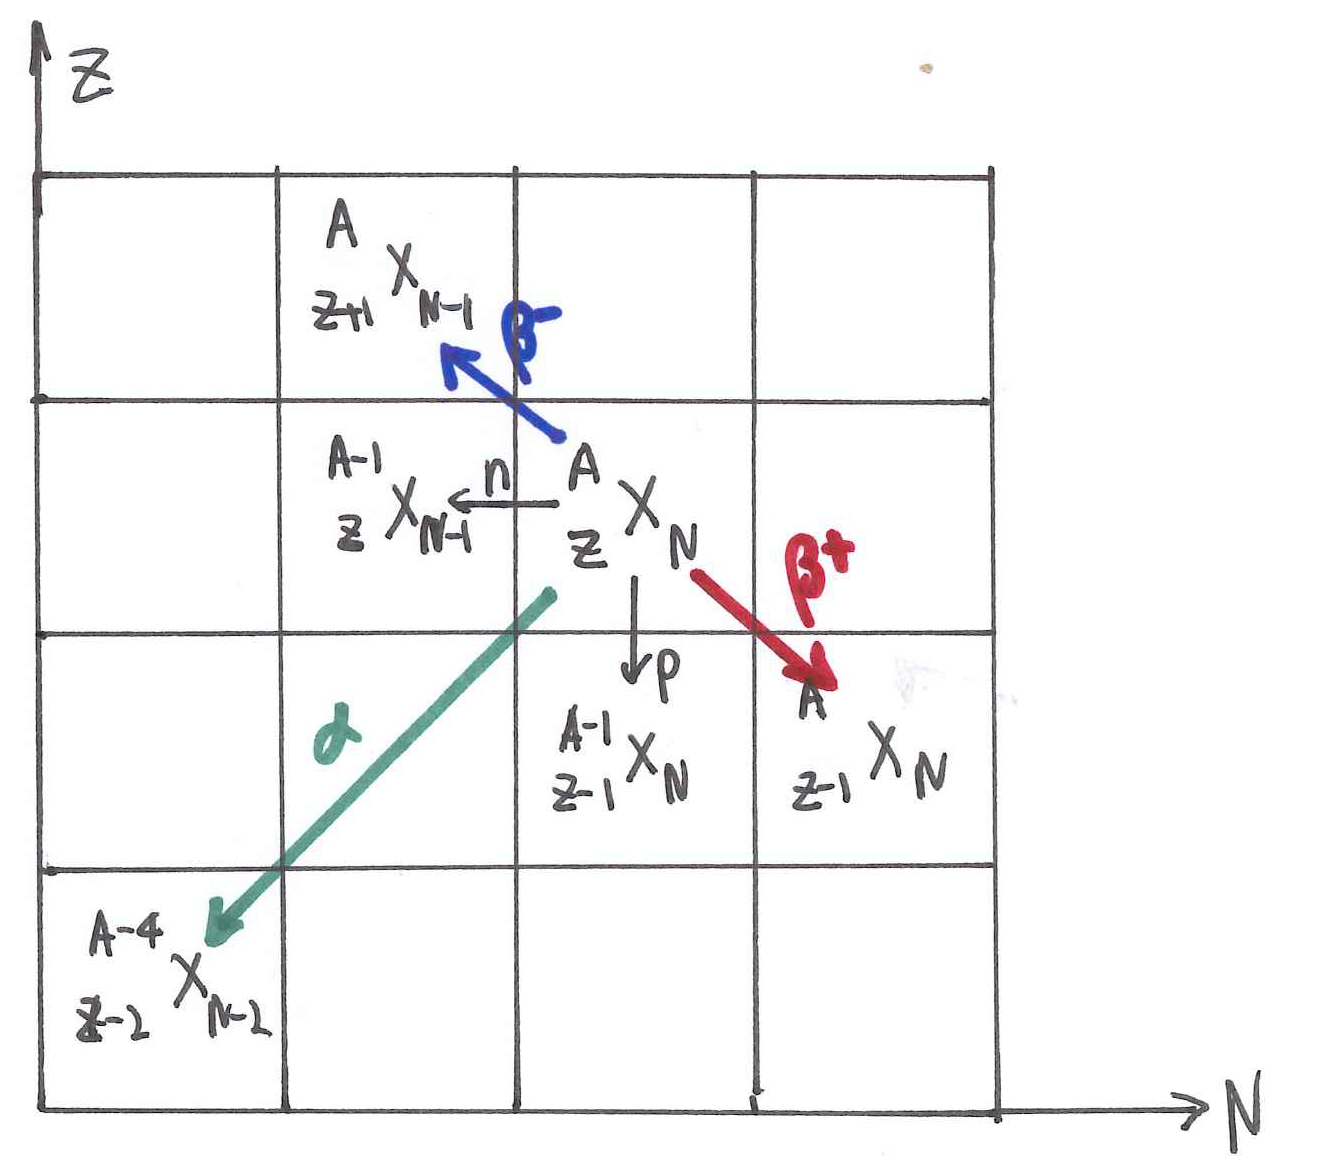
\includegraphics[width=3in]{images/rd/Z-N-grid.png}
    \end{figure}
\item Decay mechanisms: $\lambda = -\frac{\dNdt}{N(t)} =$ decay constant, describe probability of decay per unit time. It is a constant for each decay. 
    \begin{align}
    \dNdt (t) &= - \lambda N(t) &  N(t) &= N_0 e^{-\lambda  t} \\
    N(t_{1/2}) &= \frac{1}{2} N(0) & t_{1/2} &= \frac{\ln 2}{\lambda} = \frac{0.693}{\lambda} \\
    \tau &= \frac{\int_0^{\infty} t \left| \dNdt \right| \dt }{\int_0^{\infty}  \left| \dNdt \right| \dt} = \frac{1}{\lambda} & \mbox{mean lifetime} &= \frac{1}{\lambda}
    \end{align}
\item Three decay modes and their formulas. 
%%%%%%%%%%%%%%%%%%%%%%%%%%%%% Decay Summary %%%%%%%%%%%%%%%%%%%%%%%%%%%%%%%%%%%%
\begin{table}[ht]
    \scriptsize
    \begin{tabular}{|c|c|c|c|} \hline
    Properties & Alpha Decay & Beta Decay & Gamma Decay \\ \hline
    %
    \multirow{3}{*}{Notation} & \multirow{3}{*}{\ce{^A_ZX \to \ce{^{A-4}_{Z-2}\Xp} + ^4_2He} } & b.m.($n \to p$): \ce{^A_ZX \to \ce{^A_{Z+1}\Xp} + e^- + \bar{\nu}} & \multirow{3}{*}{ \ce{X^* \to X + \gamma} } \\  
    & & b.p.($p \to n$): \ce{^A_ZX \to \ce{^A_{Z-1}\Xp} + e^+ + \nu} & \\
    & & e.c. \ce{^A_ZX + e^- \to \ce{^A_{Z-1}\Xp} + \nu} & \\ \hline
    %
    \multirow{3}{*}{Mode} & \multirow{3}{*}{blank} & $\pi_P = \pi_D (-1)^L$, L = e or o? & L=e, e E, o M; L=o, o E, e M. \\
    & & $I_P = I_D + L + S$, $L_{\mathrm{min}} =$? while $S = 0,1$. & $I_P = I_D + L$, all possible L? \\
    & & For $L$, $S=0$ is Fermi, 1 is Gamow-Teller. & $L_{\mathrm{min}}$ is most probable.    \\ \hline
    %
    \multirow{3}{*}{Energy} & $m_X c^2 = m_{\Xp}c^2 + T_{\Xp} + m_{\alpha} c^2 + T_{\alpha}$ 
    & $m_X c^2 = m_{\Xp} c^2 + m_{\beta} c^2 + T_{\Xp} + T_{\beta}$ 
    & $M^* c^2 = Mc^2 + T_R + E_{\gamma}$ 
    \\ 
    & $Q = T_{\Xp} + T_{\alpha} = (m(X) - m(\Xp) - m(\alpha) )c^2$ 
    & $Q_{\beta^-} = (m(X) - m(\Xp))c^2$
    & $Q_{\gamma} =  (M^* - M)c^2  = T_R + E_{\gamma}$
    \\ 
    & $T_{\alpha} = Q \left( 1 - \frac{4}{A} \right) \approx 0.98 Q$ 
    & $Q_{\beta^+} = (m(X) - m(\Xp) - 2m_e) c^2$
    & $T_R = \frac{P_R^2}{2M} = \frac{P_{\gamma}^2}{2M} = \frac{\hbar^2 k^2 c^2}{2Mc^2} = \frac{E \gamma^2}{2Mc^2}$
    \\ \hline
    %
    %
    \multirow{3}{*}{Theory} & Gamow: barrier penetration, tunneling & Fermi: weak interaction. & Multipole transition\\
    & $\lambda = f P_T$, $E_G = \left( \frac{2 \pi e^2 Z_{\alpha} Z_D}{\hbar c} \right)^2 \frac{\mu c^2}{2}$ & $\lambda_{if} = \frac{2\pi}{\hbar} |M_{if}|^2 \rho_f$ & $\lambda = \frac{P}{\hbar \omega}$ \\
    & $2G = \sqrt{\frac{E_G}{Q}} \left[ 1 - \frac{4}{\pi} \sqrt{\frac{a}{b} } \right], P_T = e^{-2G}$ &  $N[p] = C p_e^2 (Q - T_e)^2 F(Z^{\prime}, p) |M_{fi}|^2 S(p_e, p_{\nu})$ & $P = f[L,\omega] |m_{fi} (\sigma L)|^2$ \\ \hline 
    \end{tabular}
\end{table}
%%%%%%%%%%%%%%%%%%%%%%%%%%%%% Decay Summary %%%%%%%%%%%%%%%%%%%%%%%%%%%%%%%%%%%%
\end{enumerate}

\clearpage
\uline{Alpha decay}
\begin{enumerate}
\item Conceptional stuffs:
\begin{enumerate} 
\item Why does the parent nuclei (typically heavy) want to spit out $\alpha$ particles? 

Answer: Coulomb Repulsion Effect. Coulomb force increases super-linearly with respect to binding energy\footnote{Nuclear binding energy $\propto a_V A,$ Coulomb repulsion $\propto -a_C \frac{Z^2}{A^{1/3}}$, Coulomb term increases faster than nuclear binding term for heavy nuclei.}. There is a need to get rid of some protons.  
\item $\alpha$-decay is the most favored form of radioactive decay among heavy nuclei. Very rare to observe other nucleon emission besides alpha particles. Why is the $\alpha$ particle chosen for spontaneously carrying away the positive charge?
    \begin{enumerate}
    \item \ce{^4_2 He_2} is doubly magic, very stable, tightly bound structure;
    \item \ce{^4_2 He_2} has relatively small mass compared with the mass of its separate constituents (beats \ce{^{12} C}, \ce{^{18} O}). It is favored as an emitted particle if we hope to have the disintegration products as light as possible and thus get the largest possible release of T. 
    \end{enumerate}
\item To determine whether a decay mode is possible, we need to check three things:
    \begin{enumerate}
    \item Energetically allowed, that is, $Q > 0$. Decay through emission of lighter particles is not possible because they require energy instead of release energy.
    \item $\lambda$ for the decay cannot be too small, $t_{1/2}$ cannot be too large (larger than $10^{16}$ years is no good). 
    \item Its $\beta$ decay $\lambda$ cannot be too much higher than $\alpha$ decay's, or it would mask the $\alpha$ decay. Most nuclei with $A>190$ (and many with $150 < A < 190$) are energetically possible for $\alpha$ decay, but only one-half can actually meet these requirements.
    \end{enumerate}
\item Why is decay via emission of heavier nuclei (such as \ce{^{16}O} or \ce{^{12}C}) rarely observed? 

Answer: $P_T = e^{-2G}, 2G \approx \sqrt{\frac{E_G}{Q}}, E_G \sim Z_1^2 Z_2^2$. Decaying via a heavier nuclei means $E_G$ is larger than that of $\alpha$ emission (because $Z_1, Z_2$ would be closer in value), making the probability decreases significantly. 
\item Why is decay via emission of lighter nuclei (such as \ce{^1H}, \ce{^2H}, \ce{^3He}) rarely observed?

Answer: $\alpha$ particle is favored over lighter nuclei because it is doubly magic stable, very stable, tightly bound. HW6 solution also says `this could be qualified by $Q_{\alpha}$ in $2G = \sqrt{\frac{E_G}{Q_{\alpha}}}$. 
\item Why is spontaneous fission not very likely?

Answer: spontaneous fission means $Z_1 \sim Z_2$, which makes the product large, $E_G$ large, $2G$ large, $P_T$ small. 
\end{enumerate}
%
\item Conservation of Energy:The decay will occur spontaneously only if $Q >0$. In general, $Q>0$ for $A > 150$ (but $\alpha$ decay observed for $A \ge 190$). 
\begin{align}
m_X c^2 &= m_{\Xp} c^2 + T_{\Xp} + m_{\alpha} c^2 + T_{\alpha} \\
(m_X - m_{\Xp} - m_{\alpha} ) c^2 &= B(\Xp) + B(\alpha) - B(X) =  T_{\Xp} + T_{\alpha} = Q \label{Q-alpha}
\end{align}
\item Conservation of Linear Momentum:
\begin{align}
0 &= P_{\Xp} - P_{\alpha}  & P_{\Xp}^2 &= P_{\alpha}^2 \\
T_{\Xp} m_{\Xp} &= T_{\alpha} m_{\alpha}  & T_{\Xp} &= T_{\alpha} \frac{m_{\alpha}}{m_{\Xp}} \\
Q &= T_{\alpha} + T_{\alpha} \frac{m_{\alpha}}{m_{\Xp}}  & T_{\alpha} &= \frac{Q}{1 + \frac{m_{\alpha}}{m_{\Xp}}}  \approx \boxed{ Q \left( 1 - \frac{4}{A} \right) } \approx 98\% Q
\end{align}
\item Geiger-Nuttel Rule (experimentally observed): suggesting doubling Q can result in $10^{-24}$ change in $t_{1/2}$.
\eqn{ \log t_{1/2} \propto \frac{1}{\sqrt{Q_{\alpha}}}   }
\item Gamow's Theory:
    \begin{align}
    E_G &= \left(\frac{2 \pi e^2 Z_{\alpha} Z_D}{\hbar c}\right)^2 \frac{\mu c^2}{2} = \left( \frac{2 \pi \cdot Z_{\alpha} Z_D}{137} \right)^2 \frac{m_{\alpha} m_D}{m_{\alpha} + m_D} \frac{938}{2} \\
    2G &= \sqrt{\frac{E_G}{Q}} \left[ 1 - \frac{4}{\pi} \sqrt{\frac{a}{b}} \right] \\
    P_T &= e^{-2G} \\
    \lambda &= f P_T; \fsp t_{1/2} = \frac{0.693}{\lambda} 
    \end{align}
\item Implications of Gamow's model:
\begin{enumerate}
\item Strong dependency on $Q$ because $E_G$ is so large (recall 125799 MeV for U238). Recall the graph we had that doubling $Q$ results in a $10^{20}$ change in $t_{1/2}$. 
\item The calculated $E_G$ is larger than the measured values. Potential reason: we keep the nuclear radius $a$ fixed in $x = \frac{a}{b}$ term; though for A$>$230, nuclei have strongly deformed shapes, and calculated $t_{1/2}$ is very sensitive to $x$\footnote{in fact, typically we would measure $t_{1/2}$ to reverse engineer the nuclei radius.}. 
\item Why alpha-decay not \ce{^{12} C} decay? 

Answer: If we consider $E_G \sim (Z_{\alpha} Z_D)^2 \mu c^2$, then $\frac{P_T^{\alpha}}{P_T^C} \sim \frac{\exp(-\sqrt{16})}{\exp(-\sqrt{432})} \sim \exp(16)$. `Why not spontaneous fission' can be explained similarly using Gamow's model.     
\begin{table}[ht]
    \centering
    \begin{tabular}{|c|c|c|c|} \hline
    & $(Z_{p} Z_D)^2$ & $\mu$-dependency & $P_T$ \\ \hline
    $\alpha$ &  $(2 (Z-2))^2 \sim 4Z^2$ & 3.9 & $\exp(-\sqrt{16})$ \\ \hline
    \ce{^{12} C} & $(6(Z-6))^2 \sim 36 Z^2$ & 11.4 & $\exp(-\sqrt{432})$ \\ \hline
    \end{tabular}
\end{table}
\end{enumerate}
\end{enumerate}

\clearpage
\uline{Beta decay}
\begin{enumerate}
\item Spin parity: 
    \begin{enumerate}
    \item $\pi_P = \pi_D (-1)^L$ to find whether $L$ is even or odd;
    \item $I_P = I_D + L + S$, choose lowest possible $L$ while $S = 0,1$. $L$ tells us whether the state is allowed or nth forbidden.
    \item For the lowest $L$ we find, what value can S be? $S=0$ is Fermi, $S=1$ is Gamow-Teller. 
    \end{enumerate}
\item The lowest $L$ value corresponds to the most likely state. Reason: as in $\psi_{\beta} (r) = 1 + \frac{i p_e r}{\hbar} + \frac{1}{2} \left( \frac{i p_e r}{\hbar} \right)^2 + \cdots$, the higher $L$ is, the higher order the expansion is, the less likely the term is, the smaller $\lambda$ is. Hence $\lambda_{\mathrm{allowed}} \gg \lambda_{\mathrm{forbidden}}, t_{1/2,\mathrm{allowed}} \ll t_{1/2,\mathrm{forbidden}}$. 
\item Why does beta decay's $t_{1/2}$ range from milliseconds to $10^{16}$ years? Reason: it is easy to undergo decay when $l=0$, and it is difficult to do so when $l>0$.     
\item Difference between alpha and beta decay: 
    \begin{enumerate}
    \item alpha decay has conserved neutrons and protons, use `preformed alpha-particle in daughter nuclei' theory; beta decay is transformation (\ce{n \to p}, \ce{p \to n}), creations \& annihilation of electrons and positrons.
    \item alpha decay is based on strong interaction; beta decay is based on weak interaction, transition. 
    \item $T_{\alpha}$ is a fixed value; $T_{\beta}$ is a distribution\footnote{notice we use the term $\beta$ in a weird way: $Q_{\beta} = T_{\beta} + T_{\bar{\nu}}$.}. 
    \item Parity does not conserve in beta decay.
    \end{enumerate}
\item Electrostatic results: 
    \begin{enumerate}
    \item $\beta^+$: nucleus repels $\beta^+$, KE $\up$.
    \item $\beta^-$: nucleus attracts $\beta^-$, KE $\down$. 
    \end{enumerate}
\item The energetics associated with these updated beta decays are (notice $m_n$ is nucleus mass, m is atomic mass; keep in mind $Q>0$ is the criterion for a decay to happen):
\begin{align}
Q_{\beta^-} &= \left[ m_n (\ce{^A_Z X_N}) - m_n (\ce{^A_{Z+1} X_{N+1}}) - m_e \right] c^2 = \left[ m (\ce{^A_Z X_N}) - m (\ce{^A_{Z+1} X_{N}}) \right] c^2 \\
Q_{\beta^+} &= \left[ m (\ce{^A_Z X_N}) - m (\ce{^A_{Z-1} X_{N}}) - 2m_e \right] c^2 \\
Q_{\epsilon} &= \left[ m (\ce{^A_Z X_N}) - m (\ce{^A_{Z+1} X_{N+1}}) \right] c^2 - B_n 
\end{align}
\item Fermi's Golden Rule:
\eqn{ \lambda_{if} = \frac{2\pi}{\hbar} |M_{if}|^2 \rho_f } 
\item The corrected formula for the distribution of electron momentum (which is proportional to $\lambda(p_e)$) is:
\eqn{N(p_e) = N^o (p_e) \times F(Z^{\prime},p_e) \times S(p_e,p_{\nu}) = C \underbrace{p_e^2 (Q-T_e)^2}_{\textcircled{1}} \underbrace{F(Z^{\prime}, p)}_{\textcircled{2}} \underbrace{|M_{fi}|^2}_{\textcircled{3}} \underbrace{S(p_e, p_{\nu})}_{\textcircled{4}}  }
$\textcircled{1}=$ A statistical factor derived from the density of final states available to the emitted particles; \\
$\textcircled{2}=$ Fermi function to account for the nuclear Coulomb interaction with the emitted particles;\\
$\textcircled{3}=$ Matrix element for `allowed' ($l_{\beta} = 0$) transition; strength of the interaction between initial and final states; \\
$\textcircled{4}=$ Shape factor to correct $|M_{if}|^2$ for the various `forbidden' decay paths.    
\end{enumerate}

\clearpage
\uline{Gamma decay}
\begin{enumerate}
\item Selection rule:
    \begin{enumerate}
    \item  $\pi_P = \pi_D (-1)^L$ to find whether $L$ is even or odd; if $L$ is even, then even E, odd M; if $L$ is odd, then odd E, even M;
    \item $I_P = I_D + L$, find all possible L values; write all allowed multi-poles;
    \item Most probable decay mode is lowest $L$ ($L=0$ is forbidden). 
    \end{enumerate}
    In general, magnetic multiple is weaker than electric; but as far as we are concerned, the $L$ mode dominate. 
\item Energetics (R: recoil):
\begin{align}
M^* c^2 &= Mc^2 + T_R + E_{\gamma}  & Q_{\gamma} &=  (M^* - M)c^2  = T_R + E_{\gamma} \\
|P_R| &= |P_{\gamma}| = \hbar k & T_R &= \frac{P_R^2}{2M} = \frac{P_{\gamma}^2}{2M} = \frac{\hbar^2 k^2 c^2}{2Mc^2} = \frac{E \gamma^2}{2Mc^2} 
\end{align}
A typical range of gamma energy is: $E_{\gamma} \approx 0.1 \sim 10 \fsp \MeV$. With $2Mc^2$ on the order of $2000 A$ MeV, $T_R$ is very small. Then $Q = E_{\gamma} + T_R \approx E_{\gamma}$
\item Theory ($\sigma$ is E or M): 
\begin{align}
\lambda &= \mbox{Probability per unit time for photon emission } = \frac{P}{\hbar \omega} = \frac{\mbox{Power radiated}}{\mbox{photon energy}} \\
P&= f[L,\omega] \cdot |m_{fi} (\sigma L)|^2 = \mbox{power radiated in the EM field} \cdot \mbox{multipole moment} \\
m_{fi} (\sigma L) &= \mbox{multipole transition operation} = \int_V \psi_f^* m(\sigma L) \psi_i \dV 
\end{align}
\end{enumerate}

\clearpage
%%%%%%%%%%%%%%%%%%%%%%%%% Topic 4 Neutron Interaction %%%%%%%%%%%%%%%%%%%%%%%%%%
\topic{Neutron Interaction}
\begin{enumerate}
\item Neutron energy range:
    \begin{figure}[ht]
        \centering
        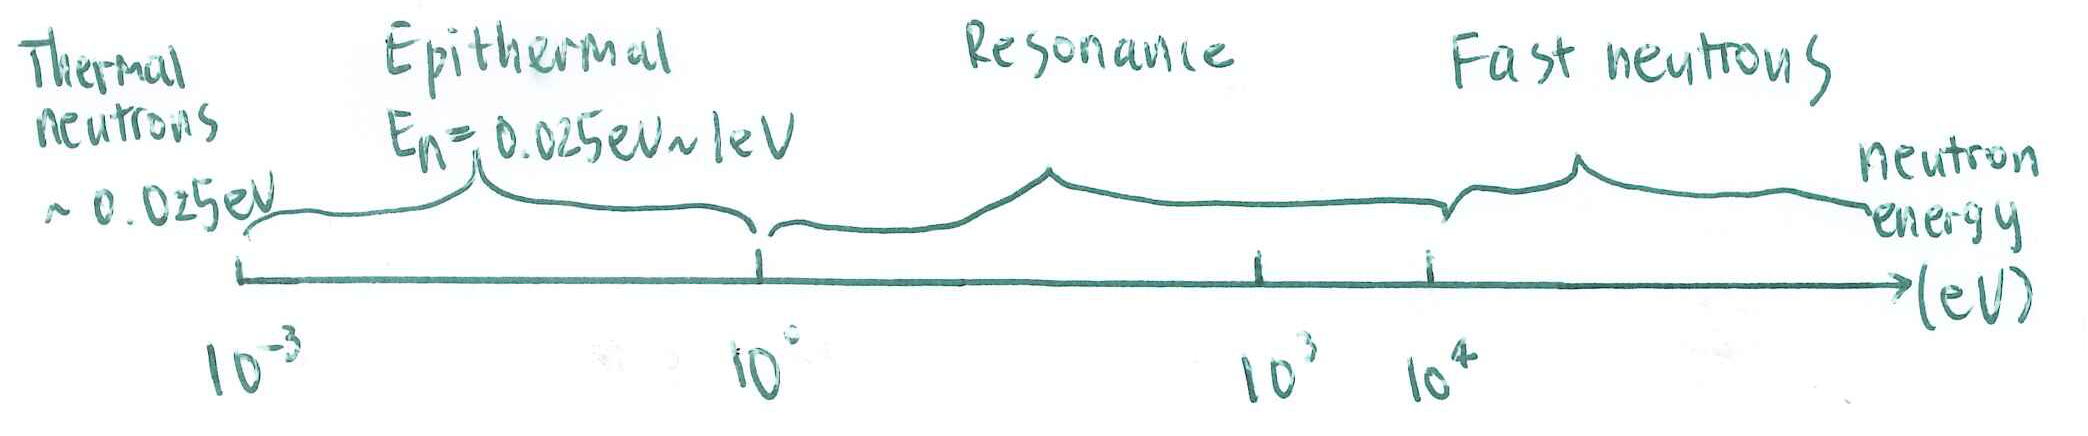
\includegraphics[width=5in]{images/ni/neutron-energy.png}
    \end{figure}
%    
\item Important neutron interactions:
    \begin{enumerate}
    \item $(n,n)$ Elastic Scattering: 
        \begin{itemize}
        \item* Potential Scattering (billard-ball like collision);
        \item Resonance Scattering (compound nucleus formation and decay);
        \end{itemize}
    \item* $(n,n^{\prime})$ Inelastic Scattering (excitation of nuclear levels);
    \item $(n, \gamma)$ Radiative Capture (get hit by a neutron, release $\gamma$ ray);
    \item $(n, p), (n,\alpha), \cdots$ Charged Particle Emission;
    \item $(n, f)$ fission.     
    \end{enumerate}
%
\item Lab CS: 
\begin{enumerate}
    \item General energetics derivation: 
    \eqn{ Q =  T_3 \left( 1 + \frac{m_3}{m_4} \right) - T_1 \left( 1 - \frac{m_3}{m_4} \right) - \frac{2}{m_4} \sqrt{m_1 T_1 m_3 T_1} \cos \theta }
    \item Elastic Scattering $\Rightarrow Q=0$ (energy lost by neutrons is energy gained by the recoiling target nucleus):
        \begin{align}
        0 &= T_3 \left( 1 + \frac{1}{A} \right)  - T_1 \left( 1 - \frac{1}{A} \right) - \frac{2}{A} \sqrt{ T_1 T_3} \cos \theta \\
        &\begin{dcases*}
        T_3^{max} = T_1 &  $\theta = 0$,  Perfect forward scattering \\
        T_3^{min} = \left( \frac{A-1}{A+1} \right)^2 T_1 = \alpha T_1 & $\theta = \pi$, Perfect backward scattering 
        \end{dcases*}
        \end{align}
    \item Inelastic Scattering $\Rightarrow Q < 0$ (energy lost by neutrons is larger than energy gained by recoiling nucleus, neutron excites the target nucleus, target nucleus gain energy through the KE of neutron):
\begin{align}
M^* c^2 - M c^2 &= E^* > 0  & M^* &= M + \frac{E^*}{c^2} \label{M*} \\
Q &= - E^* = -T_1^{min} \left( 1 - \frac{1}{A} \right) & T_1^{min} &= E^* \frac{A}{A-1} > E^* 
\end{align}
\textcolor{blue}{Minimum KE of neutron, $T_1^{min}$, is always greater than $E^*$!!!}
\end{enumerate}
%
\item CMCS: relate $E, E^{\prime}$; relate $\cos \theta, \cos \theta_C$:
    \begin{align}
     T_3 &= \frac{1}{2} T_1 \left[ (\alpha+1 ) + (1-\alpha) \cos \theta_C \right], \fsp \alpha = \left( \frac{A-1}{A+1} \right)^2 \\
    \cos \theta &= \frac{1 + A \cos \theta_C}{\sqrt{A^2 + 1 + 2A \cos \theta_C}} 
    \end{align}
Energy distribution of elastically scattered neutrons:
    \begin{align}
    P(E \to E^{\prime}) &= \frac{1}{(1-\alpha)E} \\
    \int_{\alpha E}^E (E - E^{\prime}) P(E \to E^{\prime}) \dE^{\prime} &= \mbox{Average Energy Loss per collision}  = \frac{E}{2} (1-\alpha) 
    \end{align}
Angular distribution of elastically scattered neutrons:
In CMCS the energy differential cross-section $\sigma_s(E)$ and the angular differential cross section $\sigma_s(\theta_C)$ are constant,
    \eqn{\frac{\derivative\sigma_s}{\derivative\Omega_C} = \sigma_s (\theta_C) = \frac{\sigma_s(E)}{4 \pi} }
This is not the case, however, in Lab CS (Lab CS is forward biased; though as A $\up$, distribution gets more uniform):
    \begin{align}
    \sigma_s (\theta) &= \frac{\sigma_s (E)}{4 \pi} \frac{(\gamma^2 + 2 \gamma \cos \theta_C + 1)^{3/2}}{1 + \gamma \cos \theta_C}, \fsp \gamma = \frac{1}{A}  \\
    \overline{\cos \theta} &= \frac{\int \dOmega \cos \theta \sigma(\theta)}{\int \sigma_s (\theta) \dOmega} \approx \frac{2}{3A} > 0 
    \end{align}
%
%
\item Revisit Assumptions:
\begin{enumerate}
\item Elastic Scattering Assumption: this assumption is valid when $E_n$ is small that it does not provide enough energy to excite the compound nucleus, hence the scattering from ground state of $\nu$, no energy lost for excitation. 

If $E_n > 0.05 \sim 0.1$ MeV for heavy nuclei, $E_n > 0.1 \sim 2$ MeV for medium nuclei, it would excite the first nuclear energy level above the ground state, and inelastic scattering becomes energetically possible. Elastic scattering cross section tend to be larger than inelastic scattering cross section: $\sigma (n,n) = 5\sim20$ barns, $\sigma(n,n^{\prime}) \sim 1$ barn.

\item Target at rest: this assumption is valid when neutron energy is large compared to the KE of the target nucleus ($k_B T$): $E_n \gg k_B T$. Typically, $E_n > 0.1$ eV is enough for making this assumption. 

When $E_n \approx k_B T$, neutron energy is around the same level as the thermal motion of the target, and neutron can gain energy from the vibration of the target nucleus. 
\begin{figure}
    \centering
    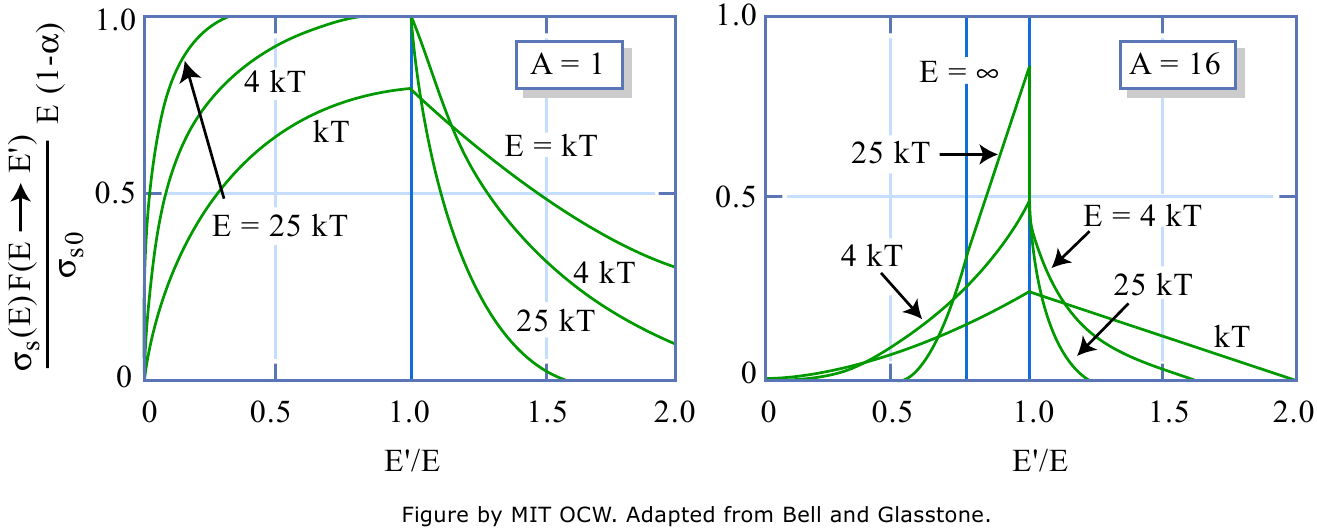
\includegraphics[width=4in]{images/ni/lower-neutron-energy.png}
\end{figure}

\item Isotropic scattering in CMCS: this assumption is valid when $E \ll 10 $keV, $l=0$, S-wave. 

However, if $E > 10$ keV, higher angular momentum (p-wave and above) would be significant, 
\begin{align}
\frac{\derivative\sigma_s}{\dtheta} &= |f(\theta)|^2 = \Sum_l f_l P_l(\cos \theta)  = \underbrace{f_0}_{\mathrm{S-wave}} + \underbrace{f_1 \cos \theta}_{\mathrm{P-wave}} + \cdots \\
\sigma_s (\theta_C) &= \frac{\sigma (E)}{4 \pi} ( 1 + a \cos \theta_C) \\
P(\Omega_C) &= \frac{1 + a \cos \theta_C}{4 \pi}, \fsp \fsp P(\theta_C) = \int P(\Omega_C) \dphi \\
P(E^{\prime}) &= \frac{1}{2} (1 + a \cos \theta_C) \sin \theta_C \frac{\dtheta_C}{\dE^{\prime}} = (1 + a \cos \theta_C) \frac{1}{E(1-\alpha)} \\
&= \frac{a}{\mbox{constant}} + \frac{2 a E^{\prime}}{(1-\alpha)^2 E^2}
\end{align}
\begin{figure}
    \centering
    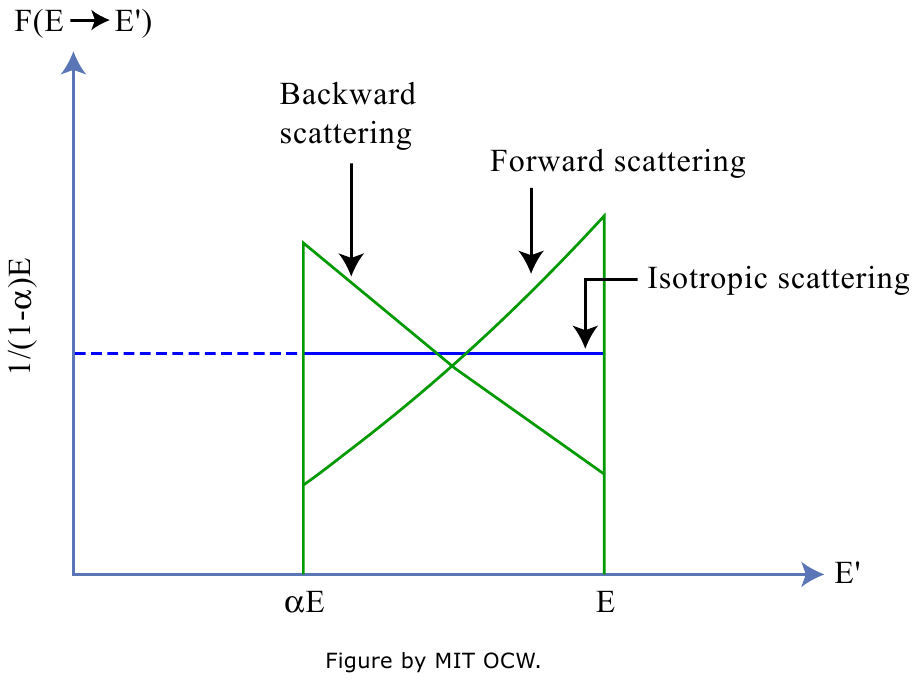
\includegraphics[width=3in]{images/ni/p-wave-approx.png}
\end{figure}
\end{enumerate}


\item Energy Dependence of Scattering Cross-sections:
\begin{enumerate}
\item Low energy range ($E \le 1$ eV): neutrons can feel the thermal motion of the target nuclei; under 0.01 eV, neutron can see molecules; above it, neutrons can see atoms.
    \begin{align}
    \sigma_s (v) &= 
    \begin{dcases*}
    \mbox{constant } \frac{\sigma_{so}}{v}& $E \ll k_B T, \beta \ll 1$ \\
    \mbox{constant } \sigma_{so}, \mbox{E independent, isotropic} & $E \gg k_B T, \beta \gg 1$ 
    \end{dcases*} 
    \end{align}
\item Oscillation in the low energy range: Bragg-cutoff corresponds to the lattice parameter, and every spikes afterwards correspond to smaller lattice spacings. 
\item S-wave potential scattering: constant.
\item Resonance region: Compound Nucleus Formation, describes elastic resonance scattering, inelastic scattering, radioactive capture, fission. 
\end{enumerate}

\item Fission
\begin{enumerate}
\item Based on $Q$ and $V^{\mathrm{peak}}$ relation:
    \begin{enumerate}
    \item $Q \sim V^{\mathrm{peak}}$: spontaneous fission, use Tunneling; 
    \item $Q > V^{\mathrm{peak}}, A>300$: instantaneous spontaneous fission (rare);
    \item $Q < V^{\mathrm{peak}}$: induced fission, provide help/energy to climb over the coulomb barrier (called Activation Energy). 
    \end{enumerate}
    \begin{figure}[ht]
       \centering
       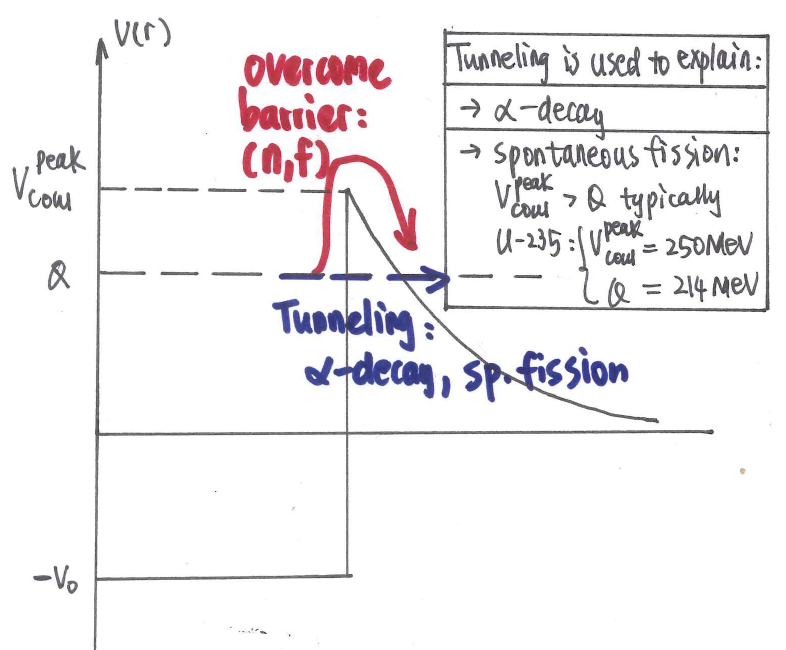
\includegraphics[width=3in]{images/ni/fission-mechanism.png}
    \end{figure}
\item Why is spontaneous fission not very common? 

Answer: Use \ce{^{238}_{92}U \to 2 ^{119}_{49}Pd + (n, \beta, \gamma, KE) }  as an example, the energy release can be calculated from binding energy
\eqn{ Q = 238 \times \underbrace{(-7.6 \fsp \MeV)}_{B/A \fsp \mathrm{U}} - 2 \times 119 \times \underbrace{(-8.5 \fsp \MeV)}_{B/A \fsp \mathrm{Pd}} = -1809 + 2023 = 214 \fsp \MeV  }
The Coulomb barrier can be estimated as:
\eqn{ V = \frac{Z_1 Z_2 e^2}{R} \approx 250 \fsp \MeV}
The barrier is higher than the available energy 250 MeV $>$ 214 MeV, making tunneling probability very small. 
\item Know how to compare U235 and U238. $E_{\mathrm{excitation}} = (m_P - m_D)c^2, E_{\mathrm{activation}} = $look up table. 
\begin{table}[ht]
    \centering
    \begin{tabular}{|c|c|c|} \hline
    & U235 & U238  \\ \hline
    $E_{\mathrm{excitation}}$ & 6.54 MeV & 4.8 MeV \\ \hline
    $E_{\mathrm{activation}}$ & 6.2  MeV & 6.6 MeV \\ \hline
    To overcome barrier & Thermal n suffice & MeV energy n needed \\ \hline
    \end{tabular}
\end{table}
The difference in the excitation energies can be understood in terms of $\delta$, the paring energy term in SEMF. \ce{^{236}U} has higher $E_{\mathrm{ex}}$ upon paring, allowing it to jump over barrier easier; whereas \ce{^{239}U} has lower $E_{\mathrm{ex}}$ upon paring, requiring higher neutron energy to fission. 
\begin{figure}[ht]
   \centering
   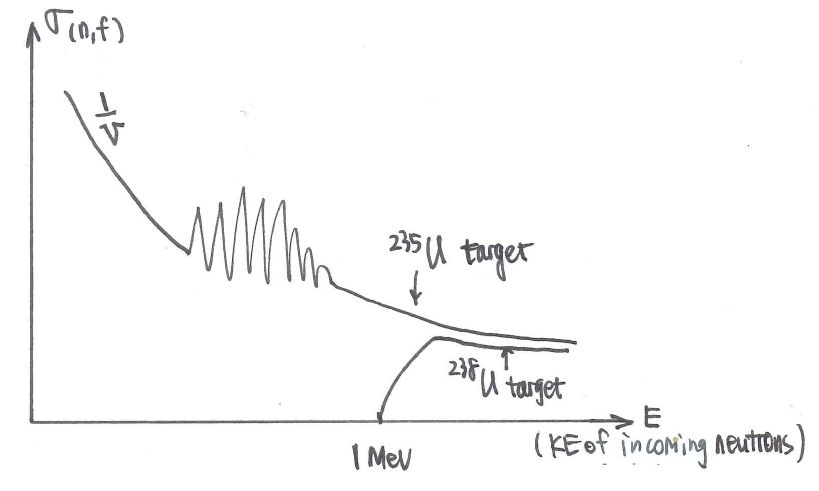
\includegraphics[width=4in]{images/ni/KE-incoming-neutron.png}
\end{figure}
\end{enumerate}

\item Fusion
\begin{enumerate}
\item The mutual Coulomb repulsion between light nuclei must be overcome before they can combine. Overcoming the barrier is not really an option (require very high temperature or heavy icon acceleration), so quantum tunneling is our only chance. 
\item Basic Fusion Reactions: 
\begin{enumerate}
\item \ce{p + p \to \ce{^2He}} (not stable, reaction not possible); 
\item \ce{p + p \to \ce{^2H} + e^+ + \nu} (first step in solar fusion, analogus to beta decay);
\item \ce{^2 H + ^2 H \to \ce{^3He} + n}, Q = 3.3 MeV ($Q>0$, hence possible); 
\item \ce{^2 H + ^2 H \to \ce{^3H} + p}, Q = 4.0 MeV (probable);
\item \ce{^2H + ^3H \to \ce{^4He} + n}, Q = 17.6 MeV (probable, larger Q than D-D reaction, ideal choice).
\end{enumerate}
\item Energy release: the lighter the particle, the more released Q it carries. For instance, in D-T reaction, KE of neutron is 14.1 MeV, total Q = 17.6 MeV, neutron carries 80\% Q.
\item Coulomb barrier: $Z_1 Z_2 \down \down, P_T \up \up$:
\begin{align}
V_{\mathrm{coul}} &= \frac{Z_{a} Z_{X} e^2 }{R} & G &\sim \frac{Z_a Z_x}{\sqrt{Q}} \\
P_T &\sim e^{-2G} \sim e^{- \frac{Z_a Z_X}{\sqrt{Q}}} & \sigma_{\mathrm{fusion}} &\sim \frac{1}{v^2} P_T
\end{align}
\end{enumerate}
\end{enumerate}


%%%%%%%%%%%%%%%%%%%%%%%%%%% A Condensed Version %%%%%%%%%%%%%%%%%%%%%%%%%%%%%%%%
\topic{A Condensed Version}
\begin{enumerate}
\item CGS unit: $\hbar c = 200 \fsp \MeV \cdot \fm$; the fine structure constant $\frac{e^2}{\hbar c} = \frac{1}{137}, m_n c^2 = 938, a=(1.2 \fm) A^{1/3}. k = \frac{2\pi}{\lambda} = \frac{p}{\hbar} = \frac{E}{\hbar c}. \int_0^a \sin^2 (n \pi x) \dx = \frac{a}{2}. \frac{e^x - e^{-x} }{2} = \sin x, \frac{e^x + e^{-x}}{2} = \cosh x.$
\item $\psi(x)$ space: $\hat{p} = - i \hbar \ddx, \hat{H} = - \frac{\hbar^2}{2m} \ddxn2 = \frac{\hat{p}^2}{2m} + V.$ $\phi(k)$ space: $p = \hbar k, E_n = \frac{\hbar^2 k^2}{2m}$. 
\item Basic Time-Independent Schroedinger Equation:
\begin{align}
- \frac{\hbar^2}{2m} \ddxn2 w_n &= E_n w_n & \ddxn2 w_n &= - k_n^2 w_n & w_n &= A \sin (k_n x) + B \cos (k_n x).
\end{align}
\item Basic Time-Dependent Schroedinger Equation: keep in mind the probability of finding an eigenstate $P_n$ does not depend on time $P_n = |C_n (t)|^2 = |C_n (0)|^2$. 
\begin{align}
\psi(x,t) &= \Sum C_n (t) w_n (x) & C_n (t) &= C_n (0) e^{-\frac{i E_n t}{\hbar}}  & C_n &= \int w_n^* \psi \dx  & \expect{E} &= \Sum P_n E_n 
\end{align}
\item Deuteron:
    \begin{enumerate}
    \item $l=0$ is the only bound state because: $V_{\mathrm{eff}} = V + \frac{\hbar^2 l(l+1)}{2 \mu r_0^2}$. 
    \eqn{ \Delta V = \frac{\hbar^2 l(l+1)}{2 \mu r_0^2} = \frac{(\hbar c)^2 l(l+1)}{2 (\mu c^2) r^2} = \frac{(200)^2 l(l+1)}{2 (500)(2.1)^2} = 10 l(l+1) \fsp \MeV   }
    For $l=1, \Delta V = 20 \fsp \MeV > E_B = 2.2 \fsp \MeV$.
    \item Spin-spin coupling is necessary, because 
    \eqn{ V_{\mathrm{eff}} = V_0 + V_1 \frac{\expect{\hat{s}_p \cdot \hat{s}_n}}{\hbar^2} = V_0 + \frac{V_1}{2} \left[ s(s+1) - \frac{3}{2} \right] = \left\{ \begin{array}{cc} V_0 - \frac{3}{4} V_1 & S=0 \mbox{ Singlet} \\ V_0 + \frac{1}{4} V_1 & S = 1 \mbox{ Triplet}  \end{array} \right.   }
    We are given $V_T = 35$ MeV, use the `barely bound state' to find $V_S$: 
    \eqn{ \frac{\lambda}{4} = r_0 \Rightarrow k = \frac{2\pi}{\lambda} = \frac{\pi}{2 r_0}, V_S \sim E+ V_S = \frac{\hbar^2 k^2}{2m} = \frac{\hbar^2}{2m} k^2 = \frac{\hbar^2}{2m} \frac{\pi^2}{4 r_0^2} \sim 22 \fsp \MeV.}
    We plug in $V_T = 35 \fsp \MeV, V_S = 22 \fsp \MeV$ to find that $V_0 = 32 \fsp \MeV, V_1 = 13 \fsp \MeV$. 
    \item $l>0$ can only exist for $s=1$, singlet well is less deep than triplet.     
    \end{enumerate}
\item SEMF (positive $\delta$ for even-even nucleon): 
\eqn{ B[A,Z] = a_V A - a_S A^{2/3} - a_C \frac{Z(Z-1)}{A^{1/3}} - a_{\mathrm{sym}} \frac{(A-2Z)^2}{A} \pm a_p A^{-3/4} }   
\item Alpha Decay Theory:
    \begin{align}
    E_G &= \left(\frac{2 \pi e^2 Z_{\alpha} Z_D}{\hbar c}\right)^2 \frac{\mu c^2}{2} = \left( \frac{2 \pi \cdot Z_{\alpha} Z_D}{137} \right)^2 \mu \frac{938}{2} &
    2G &= \sqrt{\frac{E_G}{Q}} \left[ 1 - \frac{4}{\pi} \sqrt{\frac{a}{b}} \right] \\
    P_T &= e^{-2G}, \fsp \lambda = f P_T & t_{1/2} &= \frac{0.693}{\lambda} 
    \end{align}
\item Lab CS vs. CMCS in nuclear interaction:   
    \eqn{\mu = \frac{1+ A \mu_c}{\sqrt{ A^2 + 2A \mu_C + 1}}, \fsp \fsp \frac{E^{\prime}}{E} = \frac{A^2 + 2 A \mu_C + 1}{(A+1)^2} } 
\item Three different couplings:
    \begin{enumerate}
    \item Spin-spin coupling: 
        \begin{enumerate}
        \item (n,p) deuteron, bound and virtual states.
        \eqn{ V_{\mathrm{eff}} = V_0 + V_1 \frac{\expect{\hat{s}_p \cdot \hat{s}_n}}{\hbar^2} = V_0 + \frac{V_1}{2} \left[ s(s+1) - \frac{3}{2} \right] = \left\{ \begin{array}{cc} V_0 - \frac{3}{4} V_1 & S=0 \mbox{ Singlet} \\ V_0 + \frac{1}{4} V_1 & S = 1 \mbox{ Triplet}  \end{array} \right.   }
        \item n-p scattering, spin-spin coupling fix the $\sigma_s$ magnitude problem (plug in $E_B = 2.22 \fsp \MeV, E^*  = 0.077 \fsp \MeV$):
        \begin{align}
        \sigma(\theta) &= \frac{3}{4} \sigma_T (\theta) + \frac{1}{4} \sigma_S (\theta) = \frac{3}{4} \frac{\sin^2 \theta_T}{k^2} + \frac{1}{4} \frac{\sin^2 \theta_S}{k^2} \\
        \sigma &= \frac{4 \pi \hbar^2}{2 \mu} \left[ \frac{3}{4} \frac{1}{E_B} + \frac{1}{4} \frac{1}{E^*} \right] = 19 \fsp b
        \end{align} 
        \end{enumerate} 
    \item Higher angular momentum:
        \begin{enumerate}
        \item (n,p) deuteron, $l=0$ is the only bound case because higher angular momentum create a barrier $\Delta V = \frac{\hbar^2 l(l+1)}{2 \mu r^2} = 20 \fsp \MeV > E_B = 2.22 \fsp \MeV$. 
        \item n-p scattering, higher order terms are: $\sigma = \frac{4\pi}{k^2} \Sum (2l+1) \sin^2 \delta_l$.
        \item Revisit the isotropic assumption in CMCS elastic scattering, if $E > 10$ keV higher angular momentum (p-wave and above) would be significant:
        \begin{align}
        \sigma_s (\theta) &= |f(\theta)|^2 = \Sum_l f_l P_l (\cos \theta) = f_0 + f_1 \cos \theta + \cdots \\
        \sigma_s (\theta_C) &= \frac{\sigma(E)}{4 \pi} (1 + a \cos \theta_C)
        \end{align}
        \end{enumerate} 
    \item s-l coupling: in shell model, we use s-l coupling to explain sub-shells:
        \eqn{V_{\mathrm{nuc}} = V_0 + V_1\frac{\expect{\hat{l} \cdot \hat{s} }}{\hbar^2} = V_0 + \frac{V_1}{2} \left[ j(j+1) - l(l+1) - s(s+1) \right] = \left\{ \begin{array}{cc} V_0 - \frac{l+1}{2} V_1 & j=l-\frac{1}{2} \\ V_0 + \frac{l}{2} V_1 & j = l+ \frac{1}{2}  \end{array} \right.   }
     Keep in mind $V_0 < 0, V_1 <0$, the s-l coupling weakens the well, and for each $l$ creates an energy difference of $\Delta E = \frac{\hbar^2}{2} (2l+1)$.   
    \end{enumerate} 
\end{enumerate}


\end{document}
